\chapter{Growth technique}
\label{sec:growth}

%Introduction to SiC growth
	%Various techniques
%About sublimation and nucleation modes.
	%Growing force
	%Supersaturation
%FSGP
	%The setup
	%The substrates
	%Growth of doped material
%Sample preparation
	%Polishing
	%Contacts
	

SiC can be fabricated by several different techniques, and the different techniques are advantageous for different polytypes and applications. Some of the most common methods are \emph{sublimation epitaxy}, \emph{liquid phase epitaxy (LPE)}, \emph{chemical vapour deposition (CVD)} and \emph{physical vapour transport (PVT)} \cite{Ivanov1999}. 

The goal when growing freestanding material is to have high quality material of large enough thickness to allow the substrate and transition layer to be polished away. Up to this point in time, researchers have had more success fabricating high quality 4H-SiC and 6H-SiC material compared to 3C-SiC \cite{J.B.CASADYandR.W.JOHNSON1996}. The hexagonal polytypes are commonly fabricated using PVT. This method has not been widely adapted to 3C-SiC growth however, which is often attributed to the fact that this method uses homoepitaxy, and there are no 3C-SiC seeds widely available. Nishino et al. reported in 1983 a growth rate of approximately 2.5 microns per hour with the CVD technique for 3C-SiC growth \cite{Nishino1983}. This rate is much too low to create free standing material. The growth rate for CVD growth has been improved since this time, and in 2002 Nagasawa et al. reported a rate of 40 $\mu$m/h \cite{Nagasawa2002}, which makes it possible to fabricate free standing 3C-SiC. 

Another growth method is sublimation epitaxy, which was demonstrated by Lely in 1955 \cite{Lely1955}. In this method material is transferred between a source material and a substrate using sublimation. Recently there have been reports of high quality cubic SiC fabricated by sublimation growth. Growth rates as high as 500 $\mu$m/h have been reported using this method, while still growing good quality material \cite{Jokubavicius2014}. This high growth rate is obviously ideal for growth of free standing (and even bulk) material. This chapter describes in detail the sublimation method in general and more details about the setup used in this work. 
 
 \section{About sublimation and nucleation}
 \label{sec:growth:sub_nuc}
 % What is sublimation, how does it work?
 % What governs the process?
 Sublimation is the phase transition where a material transitions between solid and gas, without the intermediate liquid phase. At normal conditions SiC does not melt, but rather it sublimes. For SiC to melt a pressure of 100,000 atm and a temperature of at least 3200 $^\circ$C is required - at atmospheric pressure SiC can only sublime \cite{Scheel2003}. Sublimation of a SiC source material will give a vapour consisting of different molecules consisting of silicon and carbon, for example $\mathrm{Si, Si_2C, SiC_2}$ etc. The composition and vapour pressure of the gas can be controlled using parameters such as temperature and pressure of the ambient. 
 
If a substrate is placed in the silicon-carbon vapour, some of the material will be adsorbed on the surface of the substrate, in the form of \emph{adatoms}. When many such atoms are adsorbed at the surface they bind together, forming a \emph{nucleus} of crystal growth. In a sublimation growth setup, a source of SiC is heated, initiating the sublimation. The vapour then travels to an appropriate substrate, by the means of a heat gradient. Material is adsorbed on the substrate which forms the grown crystal. Figure \ref{fig:sublimation} shows a schematic of this process. The vapour is transported from the source to the substrate against the temperature gradient. The higher temperature is at the source. 

\begin{figure}[h]
\begin{center}
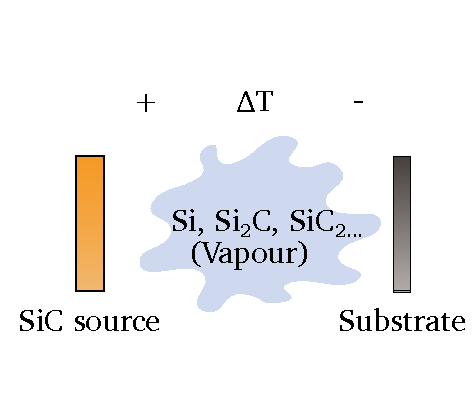
\includegraphics[scale=1]{sublimation.pdf}
\caption{A vapour containing silicon and carbon molecules is created by sublimation of a SiC source. The vapour is adsorbed at the substrate. 
\label{fig:sublimation}}
\end{center}
\end{figure}
 
 As the material is adsorbed at the substrate the growth begins. The crystal growth is governed by the free energy of the whole system. A decrease in free energy works to promote the growth. In crystal growth, a decrease in free energy is an increase in chemical potential $\mu$, meaning that crystal growth is driven by an increase in chemical potential. The system is made up by the vapour and the crystal phases, hence a change in chemical potential is given by 
 \[\Delta \mu = \mu_v -\mu_c,\]
where $\mu_v$ is the chemical potential for the vapour and $\mu_c$ is for the crystal. For growth from vapour phase, the chemical potential difference between vapour and crystal is dependent on the \emph{partial vapour pressure} and the \emph{equilibrium vapour pressure} through the formula
 \[\Delta \mu = k_BT\log(p/p_e),\]
where p is the partial vapour pressure and p$_e$ is the equilibrium (or saturated) counterpart. Defining the \emph{supersaturation}, $\sigma$, as
\[\sigma = \frac{p-p_e}{p_e}\]
thus
 \[\Delta \mu = k_BT\log(\sigma+1).\]
Taking the first order Taylor expansion this becomes
\[\Delta \mu \approx k_BT\sigma.\]
 It is concluded that the change in chemical potential is directly proportional to the supersaturation of the system. An increase in supersaturation will hence promote growth and increase growth rate. 
 
 Supersaturation is also a measure of how the crystal is formed. SiC can grown in several ways. One such way is called \emph{spiral growth}. In this growth method there are steps which originate from one point on the surface. As atoms attach to these steps, they move around the center point. This gives a spiral shape on the surface. Another way of growth is \emph{2D nucleation}. This is when atoms are adsorbed to a flat surface, and the adatoms bind to each other creating a 2D nucleus on the surface. Additional atoms will attach to this nucleus as they are adsorbed to the surface. The value of supersaturation governs which of these two methods is present. 
 
\begin{figure}[h]
\begin{center}
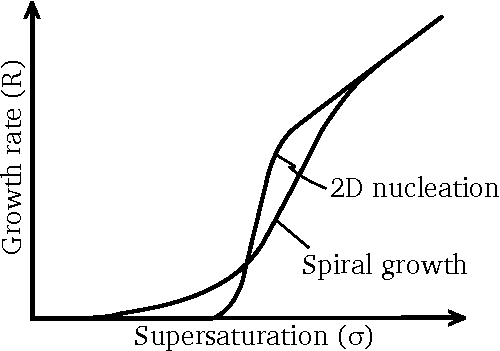
\includegraphics[scale=1]{supersaturation.pdf}
\caption{The growth rate for different modes vary depending on supersaturation. 
\label{fig:supersaturation}}
\end{center}
\end{figure}
 
 Figure \ref{fig:supersaturation} shows the general relationship between the growth rate (R) and the supersaturation ($\sigma$). It should be noted that at a certain value of $\sigma$ the growth rate of 2D growth is higher than that of spiral growth. At $\sigma$ higher than this value the 2D growth will dominate over spiral growth. 
 
\section{The sublimation growth process}
\label{sec:growth:fsgp}
The sublimation growth process used in this work is setup as shown in figure \ref{fig:fsgp_setup}. An insulating graphite foam is placed inside a quartz tube, which is surrounded by a copper coil (shown as a cutaway in the figure). The copper coil is connected to an RF-generator capable of creating a current in the coil. The foam cylinder contains a graphite crucible, which will couple with the magnetic field created by the current in the copper coil. This will heat the crucible. To measure the temperature of the crucible there is a pyrometer fixed above the quartz tube (not shown in the figure), which can measure the temperature of the crucible through a small hole at the top of the insulating foam. 

\begin{figure}[h]
\centering
\begin{minipage}{.5\textwidth}
  \centering
  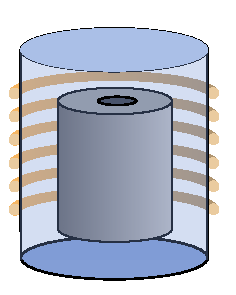
\includegraphics[scale=1]{reactor1.pdf}
  \captionof{figure}{An outside view of the reactor setup of the sublimation growht method. A copper coil surrounds a quartz tube containing an insulating graphite foam.}
  \label{fig:fsgp_setup}
\end{minipage}%
\begin{minipage}{.5\textwidth}
  \centering
  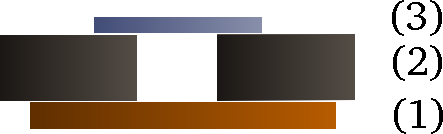
\includegraphics[scale=0.8]{undoped_growth.pdf}
  \captionof{figure}{The setup inside the crucible. (1): Polycrystalline source material, (2): Graphite spacer, (3): 4H-SiC substrate.}
  \label{fig:undoped_growth}
\end{minipage}
\end{figure}

The graphite crucible contains the components of the sublimation process, as shown in figure \ref{fig:undoped_growth}. At the bottom of the crucible is a source material, which will sublime away during the growth. When growing free-standing 3C-SiC, a polycrystalline SiC wafer piece is used as source material. The source and the substrate are separated by a graphite spacer, which is a disc with a hole in it where the vapour can flow freely. The size of the spacer and the hole can be varied depending on the desired size of the grown sample. The substrate can consist of different materials, generally 4H- or 6H-SiC. Wafers if both 4H- and 6H-SiC are commercially available and can thus readily be used as substrates in growth. When the wafers are cut, they can be cut at different angles, i.e. in different crystal planes.

Growing on on-axis substrates will give many nucleation sites. As these sites expand and merge with each other there will be many defects at the interfaces. These defects are called \emph{double positioning boundaries (DBP)}. The off-axis substrates have a surface which contains many shallow steps. As the 3C-SiC has nucleated at the edge of the growth area, the nucleation site will expand laterally along the step-flow direction. This growth method is called \emph{lateral enlargement mechanism}, and is the main principle of 3C-SiC sublimation growth, after nucleation has occurred. The density of DPBs are greatly decreased in this manner. This process is described in detail by Jokubavicius et al. \cite{Jokubavicius2014}.

As described earlier in this chapter, the growth temperature and pressure are vital parameters to determine growth rate and thus also crystal quality. In sublimation growth these parameters can easily be controlled during growth. The temperature is controlled by modulating the current from the RF-generator. A temperature ramp up scheme is used to facilitate proper step flow growth. The growth starts by homoepitaxial spiral growth of 4H-SiC on the substrate, until the supersaturation has become large enough for 2D-growth to occur. This is in accordance with figure \ref{fig:supersaturation}. It has been shown that the temperature window for 3C-SiC growth is rather narrow \cite{Vasiliauskas2012}, hence proper control of the temperature is vital for good quality material. Another important parameter is the pressure in the reactor during growth. To avoid inclusions of foreign material in the crystal a low pressure during growth is required. Typically a pressure of $10^{-4}$ to $10^{-5}$ mbar is used, which is achieved with dynamic vacuum. Some nitrogen inclusions will be unavoidable even at these pressures. A residual N-doping in the order of $10^{16}$ cm$^{-3}$ has been shown in material grown under these conditions \cite{Jokubavicius2014}, which can be compared to $10^{22}$ cm$^{-3}$ silicon or carbon atoms in the crystal. 

For a good quality crystal to form, the proper ratio between silicon and carbon must be present in the vapour. To avoid the problem with excess of carbon, a \emph{carbon getter material} is often used. This is a material which binds carbon from the vapour, thus reducing the C/Si ratio. One such material is tantalum. 

\subsection{Doping using sublimation growth}
\label{sec:growth:fsgp:doping}
It is possible to grow intentionally doped material using the sublimation growth method. To do this, the pure SiC polycrystalline source is exchanged for a doped source with the appropriate dopant density. The vapour from the sublimation will then contain the dopant element. Figure \ref{fig:direct_doping} shows the crucible setup for growth of doped material. Here the substrate contains a 3C-SiC seed before the growth starts. This is to facilitate cubic growth. 

\begin{figure}[h]
\centering
\begin{minipage}{.5\textwidth}
  \centering
  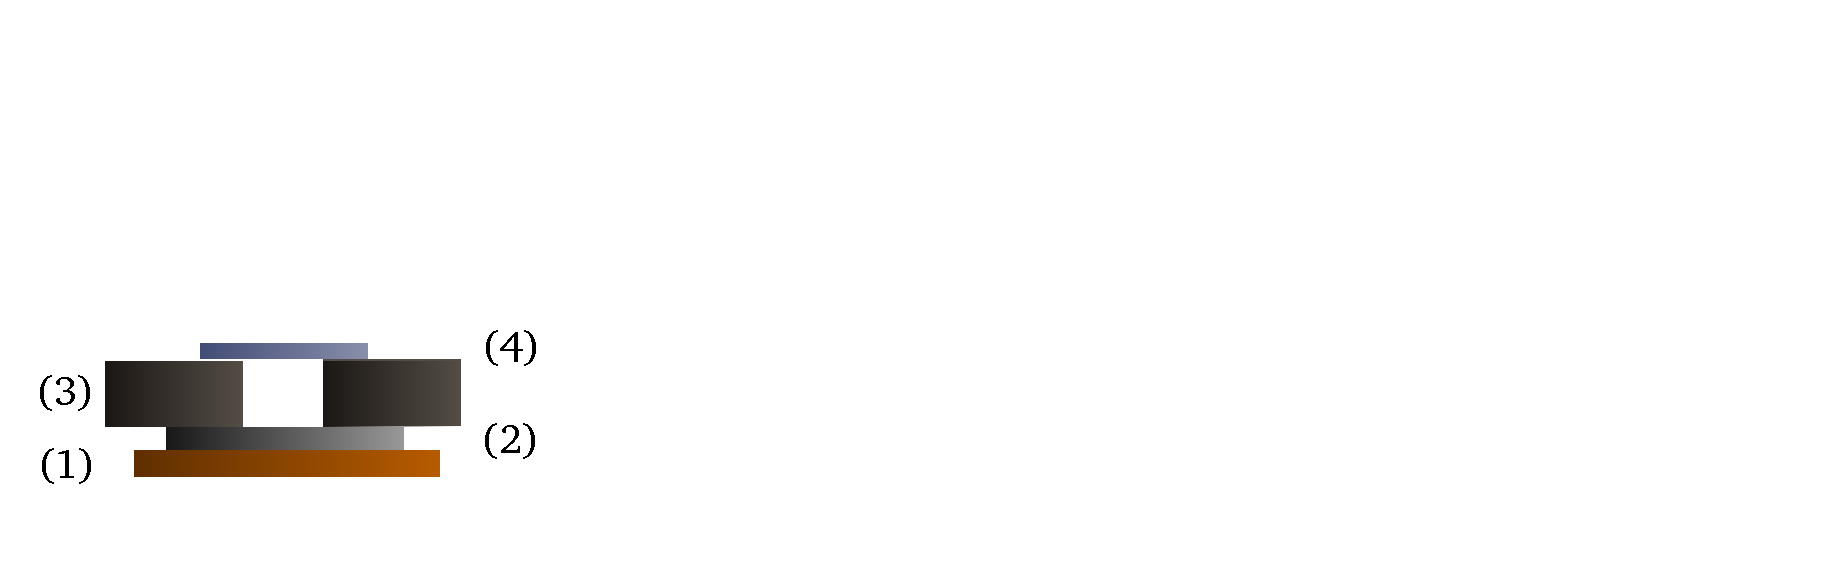
\includegraphics[scale=0.7]{doped_growth.pdf}
  \captionof{figure}{The crucible setup when doing doped growth. The source and seed (4) is separated by a graphite spacer (3) from the doped (2) and undoped (1) source material.}
  \label{fig:direct_doping}
\end{minipage}%
\begin{minipage}{.5\textwidth}
  \centering
  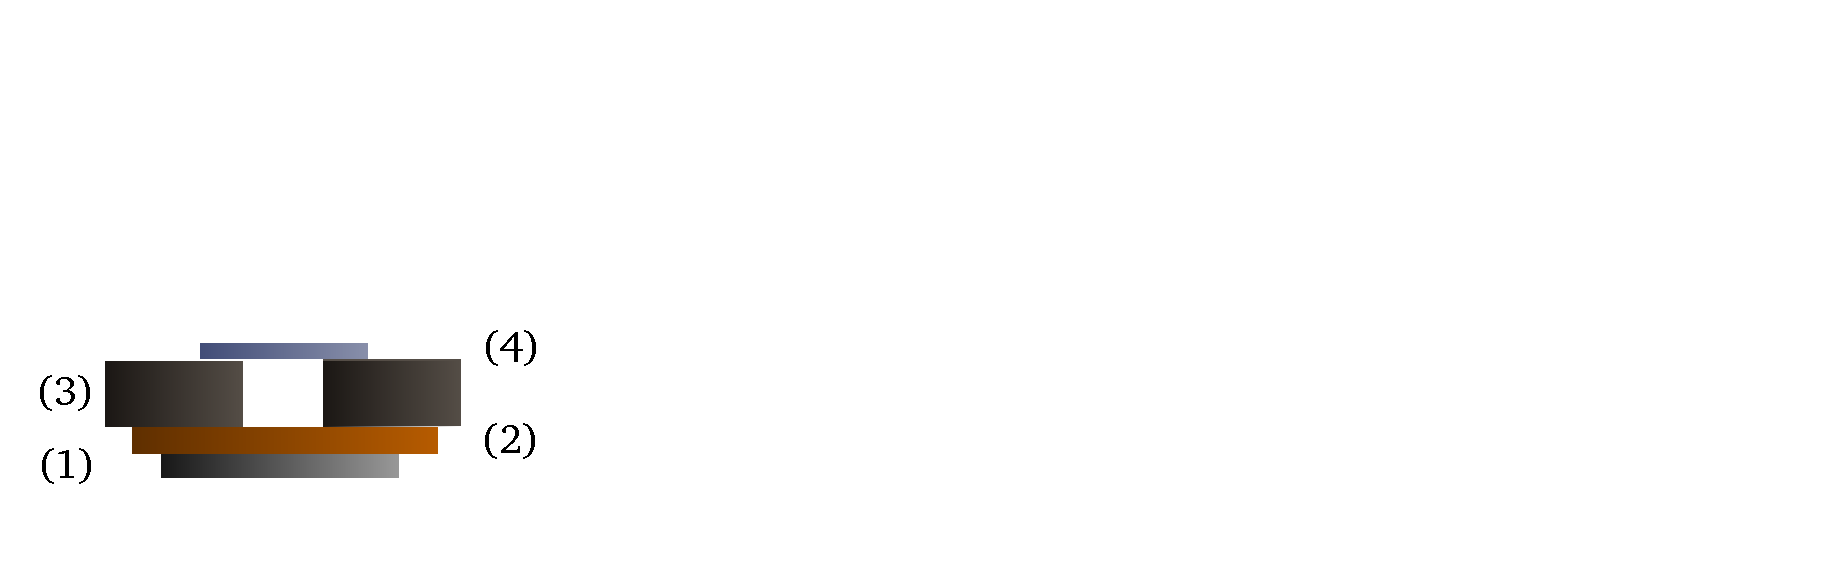
\includegraphics[scale=0.7]{indirect_doped_growth.pdf}
  \captionof{figure}{Indirect growth. Here the doped (1) and undoped (2) source materials have changed places as compared to direct growth.}
  \label{fig:indirect_doping}
\end{minipage}
\end{figure}

It is now vital to have the proper ratio between all of the elements in the vapour phase, i.e. silicon, carbon and dopant. In this thesis a new method to possibly alter this ratio is introduced. This method is called \emph{indirect doping}, and is shown in figure \ref{fig:indirect_doping}. This differs from the direct doping shown in figure \ref{fig:direct_doping} in that the doped source is now separated from the substrate by a nominally undoped source layer. If the doped source material is not homogeneous, the indirect method is hoped to give a better grown material, as well as reduce the dopant content in the vapour. 

%On/off axis substrates
%Growth temperatures?
	%Temperature gradients
	%Vacuum
%Doped growth
	%Indirect doping growth process
	
\section{Contact attachment}
This section will describe how contacts are attached to the samples. 




 
 
 %Do I really want this text?
 %Growth of the crystal can occur in several ways. One such way is called \emph{lateral enlargement} or simply \emph{lateral growth}. This growth mode is present on smooth surfaces. For growth to occur there must exist a place where the adatoms can bind to the surface. One such place is at a step on the surface. Steps on the surface will contain \emph{kinks}, which can be described as corners in the step. An adsorbed adatom diffuses on the surface until it encounters such a step kink, where it attaches. As atoms are bound to the step, it moves forward with a certain velocity. This velocity can be shown, as is done in \cite{Scheel2003}, to be
%\[v_{\infty} = \frac{2\lambda_s}{n_0}\frac{p_e}{\sqrt{2\pi mk_BT}}\sigma.\]

%Here $\lambda_s$ is the diffusion length of an adatom before it gets desorbed from the surface. Moreover $n_0$ is the density of lattice points on the surface and m is the atom mass. It is important to note that the step velocity, and hence the growth rate, is linearly proportional to the supersaturation. A high supersaturation is good for high growth rate, but there is also a disadvantage with high supersaturation. This is that at high supersaturation the time it takes for a nucleus to form is very short, which will give a material which is not a single crystal. 
 
 
% \section{Growth using FSGP}

 


 
 
 
 
 
 
 
 
 
 
 
 
 
 
 
 
 
 
 
 
 
 
 
 
 
 
 
 
 
 
 
 
 
 
 
 
 
 
 
 
 
 
 